\documentclass[conference]{IEEEtran}

\usepackage{graphicx}
\usepackage{amsmath}
\usepackage{booktabs}
\usepackage[hidelinks]{hyperref}
\graphicspath{{figs/}}

\title{Autograd from scratch: from the chain rule\\ to the curvature of a trained network}
\author{\IEEEauthorblockN{Pranav Kumar}
\IEEEauthorblockA{University of California, Irvine\\
\texttt{pkumar4@uci.edu} \quad \texttt{github.com/krrpranav/autograd-from-scratch}}}

\begin{document}
\maketitle

\begin{abstract}
I wanted to know what actually happens when you call \texttt{loss.backward()}. So I built
it, in pure NumPy, with no \texttt{torch.autograd} anywhere in the engine. This is a record
of that build. It starts where Karpathy's \texttt{micrograd} starts, a scalar reverse-mode
engine, and goes a good deal further: a tensor engine with broadcasting, forward mode as
well as reverse, a proof that the two modes are adjoints of one another, exact second
derivatives, differentiation through an optimizer's solution, Hessian-vector products
without ever forming the Hessian, and finally a measurement of the curvature of a network
the engine itself trained. Every gradient is checked against PyTorch to machine precision,
and one command reproduces every number and figure here. None of the techniques are new;
the point was to understand them by building them. This is a record of what building it
taught me.
\end{abstract}

\section{Why build this}

Halfway through learning deep learning the usual way, working through a specialization and
training models with PyTorch, I kept hitting the same wall. I could write a training loop,
but I could not have told you what \texttt{backward()} really did. It was a box that
produced gradients. Reading about backpropagation did not fix this. The only thing that
ever fixes it, for me, is building the box.

So the rule I set was simple: no \texttt{torch.autograd} in the engine. PyTorch is allowed
in the tests, and only there, as a reference to check my gradients against. Everything that
computes a derivative I had to write myself. What follows is the order I built it in,
because the order is the explanation.

\section{Reverse mode: the chain rule, backward}

A \texttt{Tensor} wraps a NumPy array and, when an operation produces it, stores a small
closure that knows that operation's local derivative. Calling \texttt{backward()} builds a
topological order of the graph and walks it in reverse, handing each node the gradient of
the loss with respect to its output and letting it pass gradient back to its inputs. This
is the whole idea, and on scalars it is short.

\begin{figure*}[t]
\centering

\includegraphics[width=0.86\textwidth]{reverse_mode}
\caption{Reverse mode on a tiny graph. Values flow forward; one backward pass fills every
gradient. The lesson that stuck: a value used in two places accumulates gradient from both
paths, which is why gradients are summed and not overwritten.}
\label{fig:rev}
\end{figure*}

Lifting this to tensors adds exactly one hard thing: broadcasting. When a shape like
$(C,)$ is broadcast against $(B, T, C)$ in the forward pass, the backward pass has to sum
the gradient back \emph{down} to $(C,)$. Getting that reduction exactly right, for every
op, is the difference between gradients that look plausible and gradients that match a
reference. The per-operation checks against PyTorch pass to a tolerance of \texttt{1e-7},
and there is a second, framework-free numerical gradient check on top of that. After that
I trusted the engine enough to build on it.

\section{Forward mode, and the fact that ties the two together}

Reverse mode is the famous one because training uses it. But it is only half the story. A
\texttt{Dual} number carries a value and a \emph{tangent}, a directional derivative, and
pushes that tangent forward through the same local derivatives, op by op. There is no graph
and no reverse walk. One forward pass gives a Jacobian-vector product $Jv$.

The fact that made the whole subject click for me is that forward and reverse mode are not
two different algorithms. They are two directions of evaluating one linear map, the
Jacobian $J$. Forward mode computes $Jv$; reverse mode computes $J^{\top}u$. For any $u$
and $v$ they must satisfy
\[
\langle u,\; Jv \rangle \;=\; \langle J^{\top}u,\; v \rangle.
\]
If my forward and reverse code disagree by even a little, this identity breaks immediately,
so I get a correctness oracle for free, one that does not depend on PyTorch at all. The test
suite requires the gap to fall below \texttt{1e-10}; in practice it is floating-point zero.
I came to trust it more than any single per-op test, because it cross-examines both modes
against each other at once.

\begin{figure*}[t]
\centering

\includegraphics[width=0.9\textwidth]{forward_vs_reverse}
\caption{The same function, two directions. Forward mode seeds a tangent at the input and
carries $Jv$ to the output; reverse mode seeds a cotangent at the output and carries
$J^{\top}u$ back to the input. They are adjoints, which is why the inner-product identity
holds.}
\label{fig:adj}
\end{figure*}

The two modes also have opposite costs, and I wanted to see that rather than take it on
faith. Building the full Jacobian with forward mode costs about one pass per input; with
reverse mode, about one pass per output. So I timed both as I swept the input and output
dimensions (Fig.~\ref{fig:cross}). With outputs fixed, forward-mode cost climbs with the
number of inputs while reverse stays flat, and the two cross right where inputs equal
outputs. That crossover is the entire reason training, with its one scalar loss and millions
of parameters, lives on the reverse side.

\begin{figure*}[t]
\centering

\includegraphics[width=0.92\textwidth]{mode_crossover}
\caption{Measured cost of a full Jacobian on the engine. One mode rises with the swept
dimension while the other stays flat, crossing where inputs equal outputs. The absolute
milliseconds are machine-dependent; the shape is the point.}
\label{fig:cross}
\end{figure*}

\section{Second order, and differentiating through an optimizer}

Carrying a \emph{second} tangent through the same machinery gives exact second derivatives,
with no finite-difference error. For a scalar function, seeding the first tangent with a
direction $v$ makes the output's second tangent exactly the directional curvature
$v^{\top}Hv$. That curvature is what Newton's method needs, so the second-order engine ends
in a small Newton optimizer. On a smooth bowl it reaches machine precision in a few steps
where gradient descent needs about fifty. Curvature is the difference.

Then a harder one: if $x^{\star}(t) = \arg\min_x f(x, t)$, what is $dx^{\star}/dt$? The
obvious move is to unroll every optimizer step and backpropagate through all of them. You
do not have to. At the optimum the gradient is zero for all $t$, so differentiating
$\nabla_x f(x^{\star}, t) = 0$ gives
\[
H_{xx}\,\frac{dx^{\star}}{dt} + H_{xt} = 0
\;\Longrightarrow\;
\frac{dx^{\star}}{dt} = -H_{xx}^{-1} H_{xt}.
\]
One Hessian and one linear solve, no matter how many steps the optimizer ran. This is the
implicit function theorem, the trick that lets deep equilibrium models and optimization
layers differentiate through a solver. I checked it against the closed-form ridge-regression
derivative (agreement to \texttt{1e-16}) and against finite differences on a non-quadratic
problem.

\section{The two modes compose: Hessian-vector products}

The Hessian of a real network is far too large to form. But the Hessian times one
direction, $Hv$, is cheap, and it is all most second-order methods actually use. The trick,
due to Pearlmutter, is to compose the two modes the engine already has. Reverse mode gives
the gradient $g(x) = \nabla f(x)$; the derivative of that gradient along a direction $v$ is
exactly $Hv$:
\[
Hv = \left.\frac{d}{d\epsilon}\, \nabla f(x + \epsilon v)\right|_{\epsilon=0}.
\]
So I run reverse mode through a forward-mode perturbation. Concretely, I seed a
\texttt{Dual} whose primal is a reverse-mode \texttt{Tensor} and whose tangent is the
direction $v$. The forward pass produces the output's tangent, $\nabla f \cdot v$, as a
tracked \texttt{Tensor}; backpropagating that one scalar leaves $Hv$ in the input's gradient.
One combined pass, and the Hessian is never built.

\begin{figure*}[t]
\centering
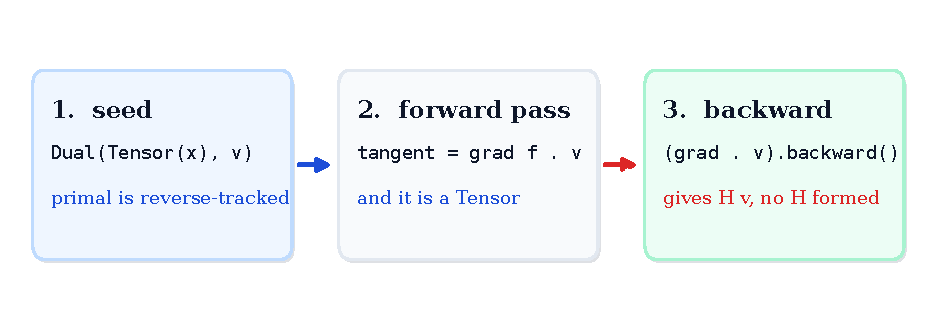
\includegraphics[width=0.92\textwidth]{hvp}
\caption{A Hessian-vector product as forward mode run through reverse mode. The part I did
not expect: I only ever wrote each operation's \emph{first} derivative. Reverse mode
differentiates that a second time on its own, so the second-order information comes out
without my writing a single second derivative by hand.}
\label{fig:hvp}
\end{figure*}

This is checked against PyTorch's double-backward, which reaches $Hv$ by a different route,
and against an explicitly-built Hessian. Both agree to machine precision (the explicit-Hessian
check to \texttt{4.4e-16}, the PyTorch one tighter still). The same $Hv$ then drives a
power-iteration for the top curvature eigenvalue and a matrix-free Newton-CG step, neither of
which forms the Hessian.

\section{Curvature of a trained network}

For a long time the second-order code only ran on toy functions I wrote by hand, which
bothered me. So the last step was to point it at a model the engine had actually trained. I
expressed a trained classifier's loss as a function of its full 1218-parameter vector and
used the engine's own Hessian-vector products to measure the sharpness of the optimum, the
largest Hessian eigenvalue, which came out near \texttt{11.8}. Walking the loss along that
sharpest direction and along a random one (Fig.~\ref{fig:land}) shows the optimum sitting
in a narrow valley: steep one way, nearly flat the other. In a 1218-dimensional space an
isotropic random direction is almost surely close to flat, which is exactly what makes it
the control.

\begin{figure}[t]
\centering

\includegraphics[width=\columnwidth]{loss_landscape}
\caption{The loss of the trained network sliced along the sharpest Hessian eigenvector
versus a random direction, both computed by the engine without forming the Hessian. A real,
measured property of a real model, read off with nothing but Hessian-vector products.}
\label{fig:land}
\end{figure}

\section{What I learned}

A few things I would not have understood without building this:
\begin{itemize}
\item Automatic differentiation is the chain rule applied mechanically, and that is all it
is. Reverse mode applies it backward, forward mode applies it forward, and second order
applies it twice.
\item The two modes are adjoints of one linear map. Once that landed, the inner-product
identity became something I could use as a test, not just admire.
\item You do not have to write second derivatives. Composing forward mode over reverse mode
produces exact $Hv$ from the first-order rules alone.
\item Curvature is a concrete, measurable property of a real loss surface, not an
abstraction, and a from-scratch engine is enough to see it.
\end{itemize}

\section{Verification}

I did not want to take any of this on trust, so every claim above is checked, mostly against
an independent reference. Table~\ref{tab:verify} collects the checks. For differentiation
code this is the strongest evidence there is: two independent implementations agreeing on
every gradient to machine precision. One command, \texttt{reproduce.py}, reruns the suite,
every demo, and regenerates every figure in this paper.

\begin{table}[t]
\centering
\caption{What is checked, against what, and how closely it agrees in the live code.}
\label{tab:verify}
\begin{tabular}{lll}
\toprule
Property & Checked against & Agreement \\
\midrule
Reverse-mode gradients & PyTorch & $< 10^{-7}$ \\
Forward mode & finite differences & $< 10^{-6}$ \\
Forward $=$ reverse & internal, no torch & f.p. $0$ \\
Second derivatives & torch double-backward & $< 10^{-8}$ \\
Hessian-vector product & torch, explicit $H$ & $\sim 10^{-16}$ \\
Implicit diff (ridge) & closed form & $10^{-16}$ \\
Parameter-space $Hv$ & dense $H$ (small net) & $< 10^{-7}$ \\
\bottomrule
\end{tabular}
\end{table}

\section{Honest scope and limitations}

I want to be clear about what this is and is not. It is a float64 NumPy engine built to be
read and understood. It is not fast, it does not use a GPU, and nobody should use it in
place of PyTorch or JAX, which do all of this and far more, faster. None of the techniques
are mine: reverse and forward mode are old, the Hessian-vector product is Pearlmutter's, the
matrix-free Newton step is the Hessian-free idea, and slicing a loss landscape along
curvature directions is a known practice. There is no new result here. What there is is one
implementation of all of it that you can read top to bottom, with every number checked
against an independent reference and one command that regenerates every figure here. The
engine ships with 68 tests; the core engine is exercised to about 98 percent.

\section{Closing}

I built this early, while I was still learning the field, and on purpose I built it from the
hard end. It would have been easier to use the gradients and move on. Writing them myself,
and then pushing past backpropagation into forward mode, the adjoint identity, second order,
and the curvature of a real network, is the reason I now actually understand the thing under
the training loop. That was the whole point.

\begin{thebibliography}{1}
\bibitem{micrograd} A. Karpathy, ``micrograd: a tiny scalar-valued autograd engine.''
\bibitem{pearlmutter} B. Pearlmutter, ``Fast exact multiplication by the Hessian,'' \emph{Neural Computation}, 1994.
\bibitem{martens} J. Martens, ``Deep learning via Hessian-free optimization,'' \emph{ICML}, 2010.
\bibitem{losslandscape} H. Li, Z. Xu, G. Taylor, C. Studer, and T. Goldstein, ``Visualizing the loss landscape of neural nets,'' \emph{NeurIPS}, 2018.
\bibitem{adsurvey} A. Baydin, B. Pearlmutter, A. Radul, and J. Siskind, ``Automatic differentiation in machine learning: a survey,'' \emph{JMLR}, 2018.
\bibitem{pytorch} A. Paszke et al., ``PyTorch: an imperative style, high-performance deep learning library,'' \emph{NeurIPS}, 2019.
\end{thebibliography}

\end{document}
